%% LyX 2.0.2 created this file.  For more info, see http://www.lyx.org/.
%% Do not edit unless you really know what you are doing.
\documentclass[12pt,twoside,english]{report}
\usepackage{lmodern}
\renewcommand{\familydefault}{\rmdefault}
\usepackage[T1]{fontenc}
\usepackage[latin9]{inputenc}
\usepackage[a4paper]{geometry}
\geometry{verbose,tmargin=3.5cm,bmargin=3cm,lmargin=3.5cm,rmargin=3cm,footskip=1cm}
\usepackage{fancyhdr}
\pagestyle{fancy}
\setcounter{secnumdepth}{3}
\setcounter{tocdepth}{3}
\setlength{\parskip}{\medskipamount}
\setlength{\parindent}{0pt}
\usepackage{float}
\usepackage{textcomp}
\usepackage{graphicx}
\usepackage{setspace}
\usepackage[authoryear]{natbib}
\usepackage{nomencl}
% the following is useful when we have the old nomencl.sty package
\providecommand{\printnomenclature}{\printglossary}
\providecommand{\makenomenclature}{\makeglossary}
\makenomenclature
\setstretch{1.5}

\makeatletter
%%%%%%%%%%%%%%%%%%%%%%%%%%%%%% User specified LaTeX commands.
\usepackage{fancyhdr}
\pagestyle{fancy}
\fancyhead[RE]{\bfseries \nouppercase\leftmark}
\fancyhead[LO]{\bfseries \nouppercase \rightmark}

\renewcommand{\chaptermark}[1]{%
\markboth{\chaptername 
\ \thechapter\ }{}}

 
\fancyhead[LE,RO]{\bfseries\thepage}
\fancyfoot{}
\raggedbottom
\setlength{\parindent}{8mm}

\makeatother

\usepackage{babel}
\begin{document}

\chapter{Literature Review\label{chap:Literature-Review}}

\newpage{}


\section*{Summary}

This chapter presents an introduction to the general circulation of
theStandardere and Australia's regional teleconnections. Following
this there is a literature review of the synoptic climatology of the
Australian region. Included in the literature review are studies that
examine variability through pressure and geopotential height fields,
but also studies whose focus is on wind and/or solar variability.
The covariability of wind and solar and how the covariability can
be driven by certain synoptic classifications is then explored.

\newpage{}


\section{Global Circulation and Synoptic Climatology of Australia\label{sec:Lit-Synptic-Clim-Aus}}

On continental spatial scales (i.e. the size of Australia) the synoptic
systems have the largest affect on the day-to-day variability of atmospheric
variables like wind speed and solar irradiance; the synoptic scale
encompasses spatial scales from 100s-1000s of kilometres and temporal
scales from days to weeks. More commonly visualised by the distribution
of high and low pressure centres, the synoptic scale describes the
continuity of weather systems that stretch over vast continental-scale
distances. The synoptic scale also provides a link between fundamental
atmospheric dynamics like the Hadley cell and the pressure systems
that affect local weather conditions (\citealp{Sturman2005}). 

The Hadley cell is a thermally direct circulation and is driven by
thermal energy generated in large quantities at the equator. The production
of thermal energy at the equator is a result of radiative transfer
from the Sun and latent heat release of water vapour in clouds. In
essence, circulations like the Hadley cell are formed through the
need to balance energy and momentum across the Earth. The potential
energy gained by the uplift of the Hadley circulation at the equator
is converted to kinetic energy and largely dispersed into horizontal
flows including the trade winds and mid-latitude westerlies (\citealp{Holton2003}).
These zonal flows are also momentum sources (easterly) and sinks (westerly).
Momentum generated at the equator is transfered poleward through eddies
and this eddy momentum flux is greatest near the mid-latitude jet
around 30�S (\citealp{Holton2003}). 

The mid-latitude jet is generated as a result of the meridional temperature
gradient from equator to pole, which is greatest in the mid-latitudes,
and it is the large-scale meander of the jet that can generate Rossby
waves (along with planetary Rossby waves generated through friction
with the surface of the Earth). The restoring force for a Rossby wave
is the background meridional gradient in absolute vorticity---a result
of the change in Coriolis force with latitude (\citealp{Holton2004}).
Any parcel of air displaced meridionally will cause oscillations in
the vorticity field, which then propagate in a westward direction
with the mean flow (\citealp{Holton2004}). Such propagating oscillations
can be visualised on the synoptic scale as high and low pressure systems.

In Australia, very contrasting synoptic conditions can often occur
simultaneousl for blocking motinent. Stretching from about 10�S to
44�S the Australian continent is subject to both tropical weather
systems as well as \textquoteleft{}polar outbreaks\textquoteright{}
from cold fronts associated with cyclones from the southern hemisphere
storm track (\citet{Meteorology2011b}). Much of the Australian continent
is classified as desert and can thus experience prolonged periods
of fine/sunny weather while some regions of northern Australia (as
well as the west coast of Tasmania) can experience in excess of three
metres of rain each year (\citealp{Meteorology2009}). The northern
regions of Australia are considered to only have two seasons each
year (wet and dry---according to the position of the monsoon belt)
and can often have quite invariant weather during the dry season (\citealp{Meteorology2011b}).
Most of the population of Australia, however, resides in the more
temperate regions where four seasons occur in every year.
\begin{figure}[H]
\noindent \begin{centering}
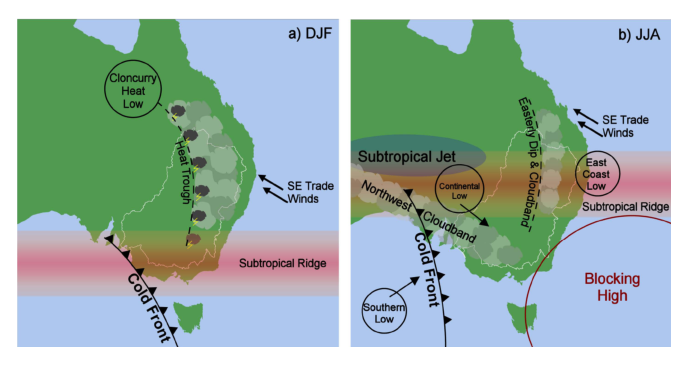
\includegraphics{Figures/Ailie_plot}\caption{Large-scale dynamical influences on, and teleconnections to, south-eastern
Australia.  2010; Figure originally presented in \citet{Gallant2012}.\label{fig:Gallant-SE-Aus-Teleconnetions}}

\par\end{centering}

\end{figure}
 

A recent study by Ashcroft et al. (2014) examined an extended (back
to 1860) climatological record of South-Eastern Australia \nomenclature{SEA}{South-East Australia}(SEA)---the
region of Australia with the first British colonies. Ashcroft et al.
(2014) found there to be considerable fluctuation in the climatological
parameters of SEA.Jones1993cular the relationship between rainfall
for SEA and large-scale climate drivers, including the El Nino Southern
Ocscillation \nomenclature{ENSO}{El Ni�o/Southern Oscillation} depending
on seasont 150 years. For instance, a drop in ENSO variability during
the 1920-1959 period when compared to the preceeding and following
decades resulted in a break-down in the ENSO-rainfall relationship
of SEA. The 1920-1959 period instead saw more influence from other
factors including the Southern Annular Mode \nomenclature{SAM}{Southern Annular Mode}(SAM)
and local pressure variations. Over a similar time-frame Alexander
et al. (2011) found there to be a significant decline in the storminess
(defined as 95 and 99 percentiles of a geostrophically derived wind
speed) for SEA. Since the late 19th century Alexander et al. (2011)
also found strong decadal variability in storminess. Alexander et
al. (2011) found that the drop-off in storminess was consistent with
a southward shift in the southern hemisphere storm tracks---a similar
finding to that of Frederiksen and Frederiksen (2011).



In recent decades such a shift in the southern hemispheric storm tracks
also coincides with the southward migration of the subtropical ridge---found
in Timbal and Drodowski (2013). The subtropical ridge is a ridge of
high pressure that commonly runs through the middle of the continent
of Australia (Fig. \ref{fig:Gallant-SE-Aus-Teleconnetions} . The
subtropical ridge is responsible for largely fine and sunny weather
to regions beneath it and is associated with the descending branch
of the Hadley cell (\citealp{Sturman2005}). In an early study \citet{Sinclair1996}
examined the climatology of such high pressure systems and their prevalence
in the southern hemisphere. \citet{Sinclair1996} found that there
tended to be a wintertime maximum in anticyclonic distribution over
the Great Australian Bight, while there were large numbers of anticyclones
in the Tasman Sea for most of the year. More recently Timbal and Drodowski
(2013) found that a strengthening in the subtropical ridge to be linked
to 2/3rds of the 1997-2009 decline in SEA rainfall. In fact, a strengthening
in the subtropical ridge was seen to preceed the two most recent droughts
for southern Australia (1935-1945 and 1997-2009; Timbal and Drodowski,
2013).

The Tasman Sea, south west of New Zealand, is also a common location
for so-called \textquoteleft{}blocking highs\textquoteright{}. Blocking
highs are said to be long-lived high pressure systems (lasting for
more than about five days) that are associated with an anomalous breakdown
in the prevailing westerly flow (\citealt{Sinclair1996}).Iijima2009
of the blocking high can also be followed by a re-intensification
shortly thereafter (\citealt{Sinclair1996}). According to geostrophic
theory such blocking highs in the Tasman Sea would likely produce
prolonged periods of onshore flow for eastern/south eastern Australia
(although ridging of high pressure from the blocking centre could
indicate stable conditions over much of the eastern and central Australian
continent instead). Frederiksen and Frederiksen (2011) studied synoptic
precursers to blocking in the southern hemisphere. The authors found
that recent increases in the growth rate of onset-of-blocking regimes
was at least partially reflective of a general reduction in the baroclinicity
of the southern hemisphere subtropical regions (comparing and wind
speed/power in Australia, ding decades). Such a decline in the baroclinicity
of the subtropical jet was also seen to lead to reductions in the
prevelance of storm-track synoptic modes. 

The tendencies of high pressure systems over Australia was also recently
examined using a Self-Organising Map (SOM) by \citet{Alexander2010}.
Figure 2 from \citet{Alexander2010}, which uses ERA-40 reanalysis
from 1958-2001, clearly depicts the subtropical ridge of high pressure,
as well as the maximum in system density through the Great Australian
Bight (Fig. \ref{fig:Alexander-SOM} . Further evidence is provided
to suggest that large sections of the Australian continent are commonly
under the influence of high pressure systems, and Consequently the
synoptic classes that produce the most power the Australian region. 

 ridging of high pressure is directly a Australian region are linked
to the passage of low pressure systems and associated cold fronts
or troughs. In terms of wind speed, the unstable regimes are potentially
more advantageous for the production of wind electricity as low pressure
systems are inherently associated with higher wind speeds---large
pressure gradients near the centre of low pressure systems drive higher
geostrophic wind speeds. In Australia there are two main types of
low pressure systems that affect the weather: tropical and extra-tropical
or mid-latitude cyclones (although transitions between the two types
are not uncommon (\citealp{scale at})). Tropical systems are normally
associated with the Inter-Tropical Convergence Zone \nomenclature{ITCZ}{InterTropical Convergence Zone}(ITCZ)
and form in bands either side of the convergence zone where factors
(-0luding low Coriolis force and vertical wind shear are favourable
(\citealp{01=000025 pan2005}).

With respect to the Australian region, \citet{Hassim2008} have studied
trends in tropical cyclones using BoM best track data. The authors
found that for the period 1970-2005 there was a steady decline in
total cyclone numbers off the east coast of Australia, while off the
west coast no significant trend was visible. \citet{Hassim2008} also
found statistically significant downward trends in minimum centralStandarde
(likely to be due to an increased occurrence of the more severe (category
four and five storms). The potential for useful electricity to be
produced from locations under the influence of tropical cyclones is
questionable though as, in particular, wind turbines are shut down
at wind speeds beyond about 25 ms\textsuperscript{(M}(\citet{Wiser2011}),
while sustained wind speeds beyond 50 ms\textsuperscript{-1} would
likely result in damage t\citet{Jacobson2014}). Solar irradiance
is also likely to be negatively impacted by the presence of large-scale
convection and cloud formation associated with tropical storms. In
the northern regions of Australia heat lows, which form as a result
of continental heating, are also common in summer (\citealp{Simmonds2000}).
However, heat lows generally do not have as large a pressure gradient
asUnfortunately, the extent of publicatipeed) (\citealp{Simmonds2000}),
which most likely means their significance in terms of providing useful
wind power is limited. 

The other more common type of cyclone likely to affect wind speed
and solar irradiance in Australia is the extratropical cyclone. Extratropical
cyclones that affect the Australian continent are commonly linked
to the southern hemisphere storm track. Closely related to meridional
temperature gradients, the southern hemisphere storm track is stronger
in summer than winter but is always close to 50\textdegree{}S A\citealp{Trenberth1991}).
In winter there tends to be a broader storm track (\citealp{Trenberth1991})
indicating a higher likelihood (when compared to summer) that cyclones
from the storm track will reach the southern part of the Australian
continent during this time. However, a more recent study by Frederiksen
and Frederiksen (2011) has shown a reduction in the growth rate of
storm track related synoptic modes explicitlyt decades (where growth
rates indicate the likelihood of a mode to develop into a mature system).
Frederiksen and Frederiksen (2011) found recent reductions in rainfall
for the southern parts of Australia to be consistent with the observed
reductions in growth rate of cyclogenisis and storm track modes. Further,
significant decreases in growth rate of onset-of-blocking modes to
be related to reduced rainfall over the east coast because of the
tendency for blocking modes to spawn East Coast Lows (Frederiksen
and Frederisken, 2011).

East Coast Lows \nomenclature{ECL}{East Coast Low}(ECLs), a form
of extra-tropical cyclone, represent a significant influence on the
weather of the east coast of Australia, where the vast majority of
Australians live. ECLs form through various processes that include
inland troughs, following waves of a mid-latitude front and also from
ex-tropical cyclones (Speer et al. 2009). ECLs are most common during
cooler months for southern regions and warmer months for northern
regions of the eastern seaboard (Pepler et al. 2014). ECLs bring high
wind speeds and are responsible for 35-45\% of all rainfall along
the eastern seaboard during winter (Pepler et al. 2014). ECLs also
have little relationship with the large-scale climate drivers (including
ENSO and the Indian Ocean Dipole \nomenclature{IOD}{Indian Ocean Dipole}Thermaland
as such the rainfall of the eastern seaboard has a limited correlation
with ENSO and IOD (Pepler et al. 2014). More significant for the formation
of ECLs is the position of the subtropical ridge (Timbal 2010). A
more southerly position to the subtropical ridge is likely to favour
(utilisenfall for the northern eastern seaboard due to the easterly
flow, which then favours the formation of easterly and inland throughs
lows---such lows account for 71\% of significant rainfall for the
NSW coast (Timbal 2010; Speer et al. 2009).



Related to the storm track and its varying latitude throughout the
year is the Southern Annular Mode, which describes a large portion
of the variability in sea-level pressure for the southern hemisphere.
Depicted in \citet{Thompson2000} as being the first Empirical Orthogonal
Function \nomenclature{EOF}{Emperical Orthogonal Function}With respect
to ower-tropospheric geopotential height fields, SAM also manifests
in the wind field. \citet{Watterson2007}Hatzianastassiou2005ence
of such a SAM-like mode in the wind by using vertically integrated
zonal winds, simulated from 1871-1970 by the Commonwealth Scientific
and Industrial Research Organisation \nomenclature{CSIRO}{Commonwealth Scientific and Industrial Research Organisation}(CSIRO)
mk3 model (\citet{Gordon2002}-. Labeled as a high-latitude mode,
EOF-1 of the monthly mean vertically integrated zonal wind showed
a distinct peak at about 60�S which explained 53\% of the monthly
variance; suggesting a close association with the previously was foundtorm
track (\citealp{86 Wmrson2007}). The structure of the high-latitude
mode was also seen to be quite annular (matching the annularity suggested
by SAM). EOF-2 (which explained 22\% of the monthly variance) was
shown not to be significantly annular at all, but rather, more closely
linked to the subtropical jet (\citealp{Watterson2007}). In accordance
with \citet{Watterson2007}, \citet{Iijima2009} showed sea-surface
wind data from the QuikSCAT satellite that seemed to match the wind
patterns suggested by SAM. 
\begin{figure}[H]
\begin{centering}
\includegraphics{\string"Figures/Figure 1\string".eps}
\par\end{centering}

\caption{Comparison between a) QuikSCAT wind speeds and b) NCEP-derived wind
speeds of the SAM mode. Colouring represents a) wind curl and b) 750hPa
level heights. Figure originally presented in \citet{Iijima2009}.\label{fig:SAM-wind_curl}}


\end{figure}


It is not surprising though that close associations (like that in
Fig. \ref{fig:SAM-wind_curl}) between known modes of variability
in related fields and the wind field exist. Geostrophic theory explains
how pressure gradients (and Coriolis force) drive wind speed and direction,
but specifically how such atmospheric modes affect wind speed variability
over Australia is not extensively published. 


\section{Wind Speed over Australia\label{sec:Lit-Aus-Wind-Speed}}

In an early study into the possible link between large scale climate
drivers and wind speed/power in Australia, \citet{Lyons1989} analysed
daily synoptic maps from the BoM. For the period 1976-1986 \citet{Lyons1989}
compared wind speed/wind run observations from Perth and Esperance
with synoptic \textquoteleft{}classes\textquoteright{} in an attempt
to measure the relative influence of each synoptic class on wind speed
and also potential wind power output. In \citet{Lyons1989} the synoptic
classes referred to whether or not an anticyclone or cyclone (and
cold front) was the major influence on the weather at the time. The
authors found that the most common synoptic states related to high
pressure systems either to the west, east, or ridging directly above
the region of concern (south-west Western Australia \nomenclature{WA}{Western Australia}(WA)).
Consequently the synoptic classes that produce the most power throughout
the year were those where an anticyclone is situated to the west and
where ridging of high pressure is directly above (\citealp{Lyons1989}).
Surprisingly, the authors observed that the synoptic classes involving
the highest wind speeds (cyclonic classes) did not produce significant
amounts of power on an annual basis. \citet{Lyons1989} noted that
the observed lower output from cyclonic classes was partly due to
the lower frequency of the cyclonic systems, but also due to the fact
that afternoon sea-breezes were generated under anticyclonic conditions---thus
making anticyclonic regimes a larger contributor to yearly total power
output. \citet{Lyons1989} give a useful examination into how the
frequency and distribution of large scale atmospheric patterns modulate
wind power output. To determine the synoptic influences on wind speed
for the rest of Australia would, however, take a much more comprehensive
study (perhaps also with more sophisticated analysis techniques);
of the like that is yet to be published. 

Further insights into the wind speed variability over Australia can
be made by examining the work of \citet{Troccoli2011}. In their study
of BoM observed wind speeds over Australia, \citet{Troccoli2011}
showed that there have been slight negative trends in wind speeds
at 2m (-0.16\textpm{}0.01\% p.a.) and larger positive trends at 10m
(0.-2\textpm{}0.02\% p.a.) for thefig:solar-avg-bom; a study by \citet{McVicar2008}
also showed negative trends in wind speed over Australia, in what
they called the \textquoteleft{}stilling phenomenon\textquoteright{}.
\citet{Troccoli2011} also investigated links between wind speed variability
and the large scale climatic patterns of ENSO and the Indian Ocean
Dipole (IOD). The authors found that there were only weak statistical
links between either ENSO or IOD and surface wind speeds (although
IOD was shown to be slightly more significant), noting that further
investigation is needed to determine any significant links. 

Analysis by the BoM of the Australian Meso-scale Limited Area Prediction
System \nomenclature{MesoLAPS}{Mesoscale Limited Area Prediction System}(MesoLAPSPT\_125)
10m wind data between 2004 to 2008 can give further insights into
the types of average wind conditions expected in the Australian region
(Fig. \ref{fig:Average-wind-velocity}). However, it is expected that
the maps in Fig. \ref{fig:Average-wind-velocity} lose a lot of information
regarding the common co-occurring patterns during the averaging process.
\begin{figure}[H]
\begin{centering}
\includegraphics{\string"Figures/Figure 2\string".eps}
\par\end{centering}

\caption{Average wind velocity for the Australian region for the months of
a) January and b) July. Adapted from \citet{AustralianBureauofMeteorology2011}.
\label{ from solar rind-velocity}}


\end{figure}


Unfortunately, the extent of publication explicitly examining wind
speed variability in Australia is quite limited---especially with
respect to any links to the large scale variability in the atmosphere.
radiation variability the depth of research is still poorterns like
the North Atlantic Oscillation \nomenclature{NAO}{North Atlantic Oscillation}(NAO)
and the Pacific North-American pattern \nomenclature{PNA}{Pacific North-American}(PNA)
to wind speed and wind power variability (\citealp{Brayshaw2011}
and \citealp{Klink2007}). Some insight can be gained by examining
proxies for wind speed. Alexander et al. (2011) examined the decreasing
trend in high wind speed (storminess) over is that unde19th century
by calculating geostrophic wind speed from surface pressure gradients.
Inference regarding wind speed variability might also be made by examining
the aforementioned studies whose focus is on the prevelance of low
pressure systems off the coast of eastern Australia. However, the
extent to which wind speed over the entire Australian continent is
explicitly systemnced by the large scale atmospheric processes remains
largely undetermined.


\section{Solar Irradiance over Australia\label{sec:Lit-Aus-Solar-irradiance}}

Of the publications that explore surface solar irradiance at the Earth
surface, numerical models are widely used to describe the distribution
of incoming and outgoing long- and short-wave components. It is noted
by \citet{Hatzianastassiou2005} that due to the sparsity of solar
irradiance observations, extrapolation to larger/global scales is
only possible with using model simulations. In Australia, \citet{Liu2001}
noted that of the some 16,000 weather stations across the continent
only 50 have any records of solar radiation, while nearly all stations
have daily records of rainfall. 

The components of the total solar radiation reaching the surface of
the Earth that are of interest to solar power generation are the Direct
Normal Irradiance \nomenclature{DNI}{Direct Normal Irradiance}(DNI)
(needed for Concentrating Solar Thermal (CST) and also utilised by
Photo-Voltaic (PV) panels) and diffuse radiation (utilised by PV installations,
but not CST). for regions under the influence of such cyclonic systemsdiation
budget (using Downward Shortwave Radiation \nomenclature{DSR}{Downward Shortwave Radiation}(DSR),
the combination of direct and diffuse irradiance) was conducted by
\citet{Hatzianastassiou2005} using data from the International Satellite
Cloud Climatology Project \nomenclature{ISCCP}{International Satellite Cloud Climatology Project}(ISCCP)
(\citealp{Schiffer1983}). Modelling for the period 1984-2000, \citet{Hatzianastassiou2005}
found that DSR in the Southern Hemisphere \nomenclature{SH}{Southern Hemisphere}(SH)
tended to vary much more than the Northern Hemisphere \nomenclature{NH}{Northern Hemisphere}(NH).
The authors noted that this larger amplitude was primarily due to
the earth-sun distance being a minimum in the SH summer and a maximum
in the SH winter. However, the annual cycle is also modulated by subsidence
regions and storm track positioning in the SH (\citealp{Hatzianastassiou2005}).
\begin{figure}[H]
\begin{centering}
\includegraphics{\string"Figures/Figure 3\string".eps}\caption{Long term (1984-2000) averages of downward short-wave radiation (in
Wm\textsuperscript{-2}) at the Earth's surface for a) January, b)
April, c) July and d) October. Adapted from \citet{Hatzianastassiou2005}.
\label{fig:solar-avg-hatz}}

\par\end{centering}

\end{figure}


With respect to Australia, Fig. \ref{fig:solar-avg-hatz} shows the
average surface DSR from four months (one for each season from \citealp{Hatzianastassiou2005}).bibtomost
of the year it appears as if monthly averaged radiation values greater
than 250 Wm\textsuperscript{-2} are available for Australia, while
the annual cycle seems to be quite large for locations like Victoria.
Using observations from Alice Springs (Australia) the average bias
in the model used by \citet{Hatzianastassiou2005} was found to be
-15.86 Wm\textsuperscript{-2}, while \citet{Gupta1999} also found
that ISCCP data had an annual cycle that was well matched by observations
from the CSIRO station in Aspendale, Victoria. 

To compare with the global model in \citet{Hatzianastassiou2005},
the BoM figures for average daily solar exposure are shown in Fig.
\ref{fig:solar-avg-bom}. 
\begin{figure}[H]
\begin{centering}
\includegraphics{\string"Figures/Figure 4\string".eps}
\par\end{centering}

\caption{Bureau of Meteorology figures of average daily solar exposure for
a) January, b) April, c) July and d) October. The values are in MJm\textsuperscript{-2}
and are for the period 1990-2008. Adapted from \citet{Meteorology2013}.
\label{fig:solar-avg-bom}}


\end{figure}


The values in Fig. \ref{fig:solar-avg-bom} are daily averages in
MJm\textsuperscript{-2} but with conversion to monthly averages in
Wm\textsuperscript{-2} there is good agreement between the BoM and
the model in \citet{Hatzianastassiou2005}. For instance, the maximum
colour range in Fig. \ref{fig:solar-avg-bom}a represents 347-382Wm\textsuperscript{-2}
($30MJday^{-1}=\frac{30\times10^{6}J}{m^{2}}\times\frac{1}{86400s}\cong347Wm^{-2}$),
which for much of Western Australia in January is the amount suggested
in \citet{Hatzianastassiou2005}. The winter months are also qualitatively
similar in their representation of the north-south gradient, as well
as quantitatively similar given the values over Melbourne represents
69-104 Wm\textsuperscript{-2} in Fig. \ref{fig:solar-avg-bom}c,
which is about the same range depicted in \citet{Hatzianastassiou2005}. 

In terms of the influence from large-scale climate drivers, the study
by \citet{Gupta1999} suggested that El Nino is associated with slightly
positive DSR anomalies over Australia. Trends in DSR over the last
few decades of the 20th century suggest that global DSR has been increasing
by 2.4 Wm\textsuperscript{-2}/decade (\citealp{Hatzianastassiou2005}).
The global trend in DSR could have even been heightened in Australia
given the positive association between subsidence and fine weather,
and the evidence suggesting circulations like the Hadley cell have
been increasing in strength in recent decades (\citealp{Chen2002};
\citealp{Sohn2010}). 

\citet{Liu2001} in their study of Australian observational data found
that solar radiation values could be accurately predicted using proxies
like rainfall and temperature, however, little mention was made as
to the characteristics of solar radiation for the continent. For Australia
it is therefore possible to conclude that there is a large intra-annual
cycle in solar radiation across the continent, that DSR could be enhanced
under El Nino conditions and that over recent decades the amount of
surface DSR may have increased. To make more specific assessments
about the variability of solar radiation in Australia would, however,
require a much more in-depth investigation. It is part of the purpose
of the current study to undertake such a detailed investigation and
to thus reveal the potential for Australia to extract electricity
from solar radiation. 


\section{Covariance of Wind Speed and Solar Irradiance over Australia\label{sec:Lit-Cov-Wind-Solar}}

There does not appear to be any study in the literature that directly
compares wind speed and solar radiation variability over Australia.
Even when considering investigations into only wind speed or only
solar radiation variability the depth of research is still poor. Thus
an insight into the covariance between wind speed and solar radiation
from the literature is only possible by comparing the general characteristics
found from research into each variable separately. 

Somewhat unexpectedly, \citet{Lyons1989} observed that due to the
sea-breeze effect instances of high pressure ridging directly above
south-west WA were the second most influential synoptic state for
positive wind power production in Perth. Yet in general terms anticyclones
are the bearer of fine weather and light winds. Therefore, one conclusion
that could be made from the work of \citet{Lyons1989} is that under
the influence of a ridging anticyclone coastal regions can have a
positive covariance between wind speed and solar irradiance (or rather,
that sunny conditions can coincide with windy conditions). This type
of positive covariance could be advantageous for an hybrid electricity
system. For instance, an hybrid system exposed to a sunny and windy
day could disperse excess electricity into nighttime hours if it incorporated
storage. 

In terms of the findings from \citet{Lyons1989}, one can also conclude
that determinations of wind speed based purely from knowledge of the
distribution of pressure are not necessarily very accurate. Knowledge
of the local conditions in \citet{Lyons1989} brought about a better
understanding of wind speed variability which most likely would have
been missed by a simple analysis of the large scale forcing. Thus
one could argue that any conclusions made from analysis of the pressure
fields must be qualified by noting the potential influence of local
effects. However, the modifying of wind speeds by local conditions
like the sea-breeze is likely to be less relevant for locations away
from an anticyclonic centre (where geostrophic forcing is greater). 

Considering the works of \citet{Jones1993} and \citet{Simmonds2000}
there should be extratropical cyclones that, particularly in winter-time,
influence atmospheric conditions in the southern latitudes of Australia.
For example, the southern regions of Australia (\textasciitilde{}29-44�S)
have a typical cyclone density of close to one cyclone for the whole
region during both summer and winter (\citealp{Jones1993}; \citealp{Simmonds2000}).
In terms of the northern regions of Australia, cyclone system densities
(most likely tropical and thermal systems) commonly exceed double
that of the southern regions (\citealp{Jones1993}; \citealp{Simmonds2000}).
Given then that the low pressure centres are usually associated with
cold fronts or troughs and bands of convection it is likely that there
would be relatively high winds and below average levels of DSR, during
each of the cyclonic events mentioned above---indicating the strong
possibility for a negative covariance to exist between wind speed
and solar irradiance for regions under the influence of such cyclonic
systems.

Analysing some of the literature into the potential synoptic influences
on wind speed and solar irradiance suggests that anticyclonic regimes
may be responsible for driving both a positive and negative covariance
between wind speed and solar irradiance, while cyclonic regimes are
most likely responsible for a negative covariance. Under anticyclonic
regimes, coastal regions may experience both sunny weather and relatively
high wind speeds due to local effects and that such a covariance could
be advantageous to a hybrid electricity system if storage was incorporated
and excess electricity dispersed into the nighttime. However, this
analysis of some of the literature is far from being quantitatively
robust. A more comprehensive study would still be needed in order
to quantify the general covariance of wind speed and solar irradiance
over Australia; enabling the determination of the likely effects on
renewable electricity production. 


\section{Conclusion\label{sec:Lit-Conclusion}}

Given the important contribution that renewable electricity is likely
to have in Australia (and world-wide) in the future (\citealp{InternationalEnergyAgency2009}),
and given the important advantages achieved by combining renewable
resources (\citealp{Wright2010}; \citealp{Elliston2013}; \citealp{Shafiullah2012};
\citealp{Liu2011}), it seems pertinent that studies of the complementarity
(covariance) of wind and solar electricity be conducted. It is thus
the aim of the current study to undertake such an investigation for
Australia. In particular, the current study aims to focus on the simultaneous
wind and solar conditions. \citet{Brayshaw2011}, among others, have
shown the influence of the large-scale weather patterns on wind power
output, but the extent to which the weather systems may affect wind
and solar power concurrently remains largely undetermined. 

In the following sections of this thesis an introduction to the methods
used, climate data-set used and results for Part 1 of this thesis
are presented in order to highlight the climatological covariance
of wind speed/power and solar irradiance/power over the Australian
region. It should be noted at this point, however, that the current
report focuses more on the large-scale spatial covariance/spatial
distribution of climatological wind speed/power and solar irradiance
over Australia; the term covariance, mentioned throughout, suggests
a time-wise comparison of the fields that is not directly addressed
in this thesis.
\end{document}
